%%%%%%%%%%%%%%%%%%%%%%%%%%%%%%%%%%%%%%%%%%%%%%%%%%%%%%%%%%%%%%
\chapter{FIRSTv2 au télescope Subaru}
\label{sec:FIRSTv2Subaru}
\setcounter{figure}{0}
\setcounter{table}{0}
\setcounter{equation}{0}

\minitoc

\clearpage
%%%%%%%%%%%%%%%%%%%%%%%%%%%%%%%%
\section{La plateforme SCExAO}

\acrfull{SCExAO} \citep{jovanovic2015} est une plateforme de R\&D pour l'imagerie \acrfull{HRA}, installé sur la plateforme Nasmyth (voir la photographie de la figure~\ref{fig:SCExAOPhoto}) du télescope Japonais Subaru de $8,2 \,$m de diamètre. L'objectif primaire de la plateforme est de développer et de mettre en place un système d'optique adaptative extrême afin de fournir à plusieurs instruments un faisceau avec un haut rapport de Strehl ($80 \%$ dans la bande H). Certains de ces instruments sont accessibles à la communauté scientifique : \acrfull{CHARIS} \citep{groff2015}, \acrfull{VAMPIRES} \citep{norris2015}, \acrfull{REACH} \citep{kotani2018}, \acrfull{MEC} \citep{walter2020} et Fast \acrfull{PDI} \citep{lozi2020}. Et d'autres sont des modules permettant le développement de nouvelles solutions techniques pour l'imagerie \ac{HRA} : \ac{GLINT} \citep{norris2020b}, \ac{RHEA}\footnote{\url{https://www.naoj.org/Projects/SCEXAO/scexaoWEB/050devmodules.web/030rhea.web/indexm.html}} et \ac{FIRST}.

\begin{figure}[ht!]
    \centering
    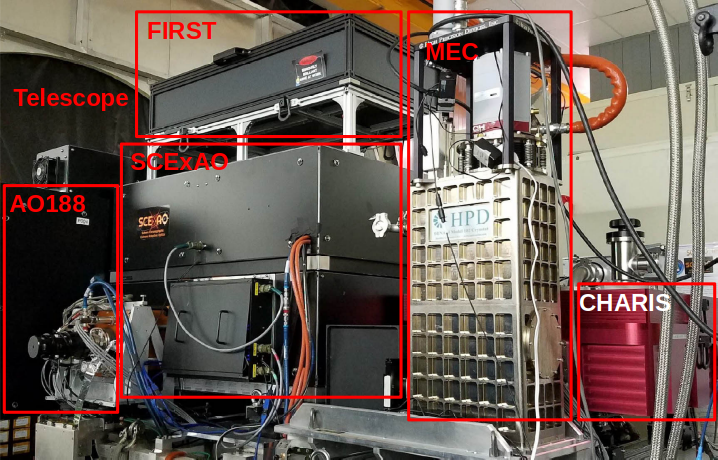
\includegraphics[width=\figwidth]{Figure_Chap5/SCExAO_onNasIR_label.png}
    \caption[Photographie de la plateforme SCExAO et des modules installés sur la plateforme Nasmyth IR du télescope Subaru.]{Photographie de la plateforme SCExAO et des modules installés sur la plateforme Nasmyth IR du télescope Subaru. Crédit : équipe SCExAO.}
    \label{fig:SCExAOPhoto}
\end{figure}

La figure~\ref{fig:SCExAOScheme} présente le schéma optique global de \ac{SCExAO}. Il est divisé en quatre blocs représentant les différents étages du banc. La lumière provenant du télescope subit une première correction appliquée par l'étage d'optique adaptative AO188 \citep{minowa2010} (module externe à \ac{SCExAO}) avec un miroir comportant $188$ actionneurs.

Le faisceau en sortie de cet étage est injecté sur le banc \ac{SCExAO} (dans le cadre du bas de la figure~\ref{fig:SCExAOScheme}) sur l'étage \ac{IR} (\textit{IR bench}), sur lequel le faisceau est divisé en deux à l'aide d'une dichroïque : un faisceau visible ($< 950 \,$nm) et un faisceau \ac{IR} ($< 950 \,$nm). Ce dernier est injecté vers les instruments travaillant dans l'\ac{IR}, indiqués par les flèches oranges sur les bords du cadre. Le faisceau lumineux passe, entre autre, par des composants (\ac{PIAA} et \textit{focal plane mask}) appliquant une correction coronographiques (voir à ce sujet la section~\ref{sec:ImagerieDirecte}).

La partie visible du faisceau est injectée sur l'étage visible (cadre du milieu nommé \textit{visible bench}) à travers un périscope. Ce faisceau est de nouveau divisé en deux sous-faisceaux. L'un d'eux ($800 - 950 \,$nm) est analysé par le senseur de front d'onde comportant une pyramide \citep{lozi2019} et permet d'appliquer la deuxième étape de correction par optique adaptative extrême à l'aide d'un miroir déformable comportant $2\,040$ actionneurs, intégré sur le banc \ac{IR}. L'autre ($< 800 \,$nm) est injecté dans les instruments travaillant dans le visible tels que \ac{FIRST}, \ac{VAMPIRES} et \ac{RHEA}.

Enfin, le cadre de gauche en haut de la figure~\ref{fig:SCExAOScheme} présente le schéma de principe des différentes sources internes, notamment la \sk~qui est injectée dans \ac{FIRST} lors des tests et de l'étalonnage de la \ac{P2VM}. L'étage de recombinaison de \ac{FIRST} est représenté par le cadre de droite. Il s'agit de sa configuration finale équivalente à celle présentée sur le schéma du bas de la figure~\ref{fig:FIRSTSubaruScheme} et qui sera présenté dans la section~\ref{sec:V1V2Subaru}.

\begin{figure}[ht!]
    \centering
    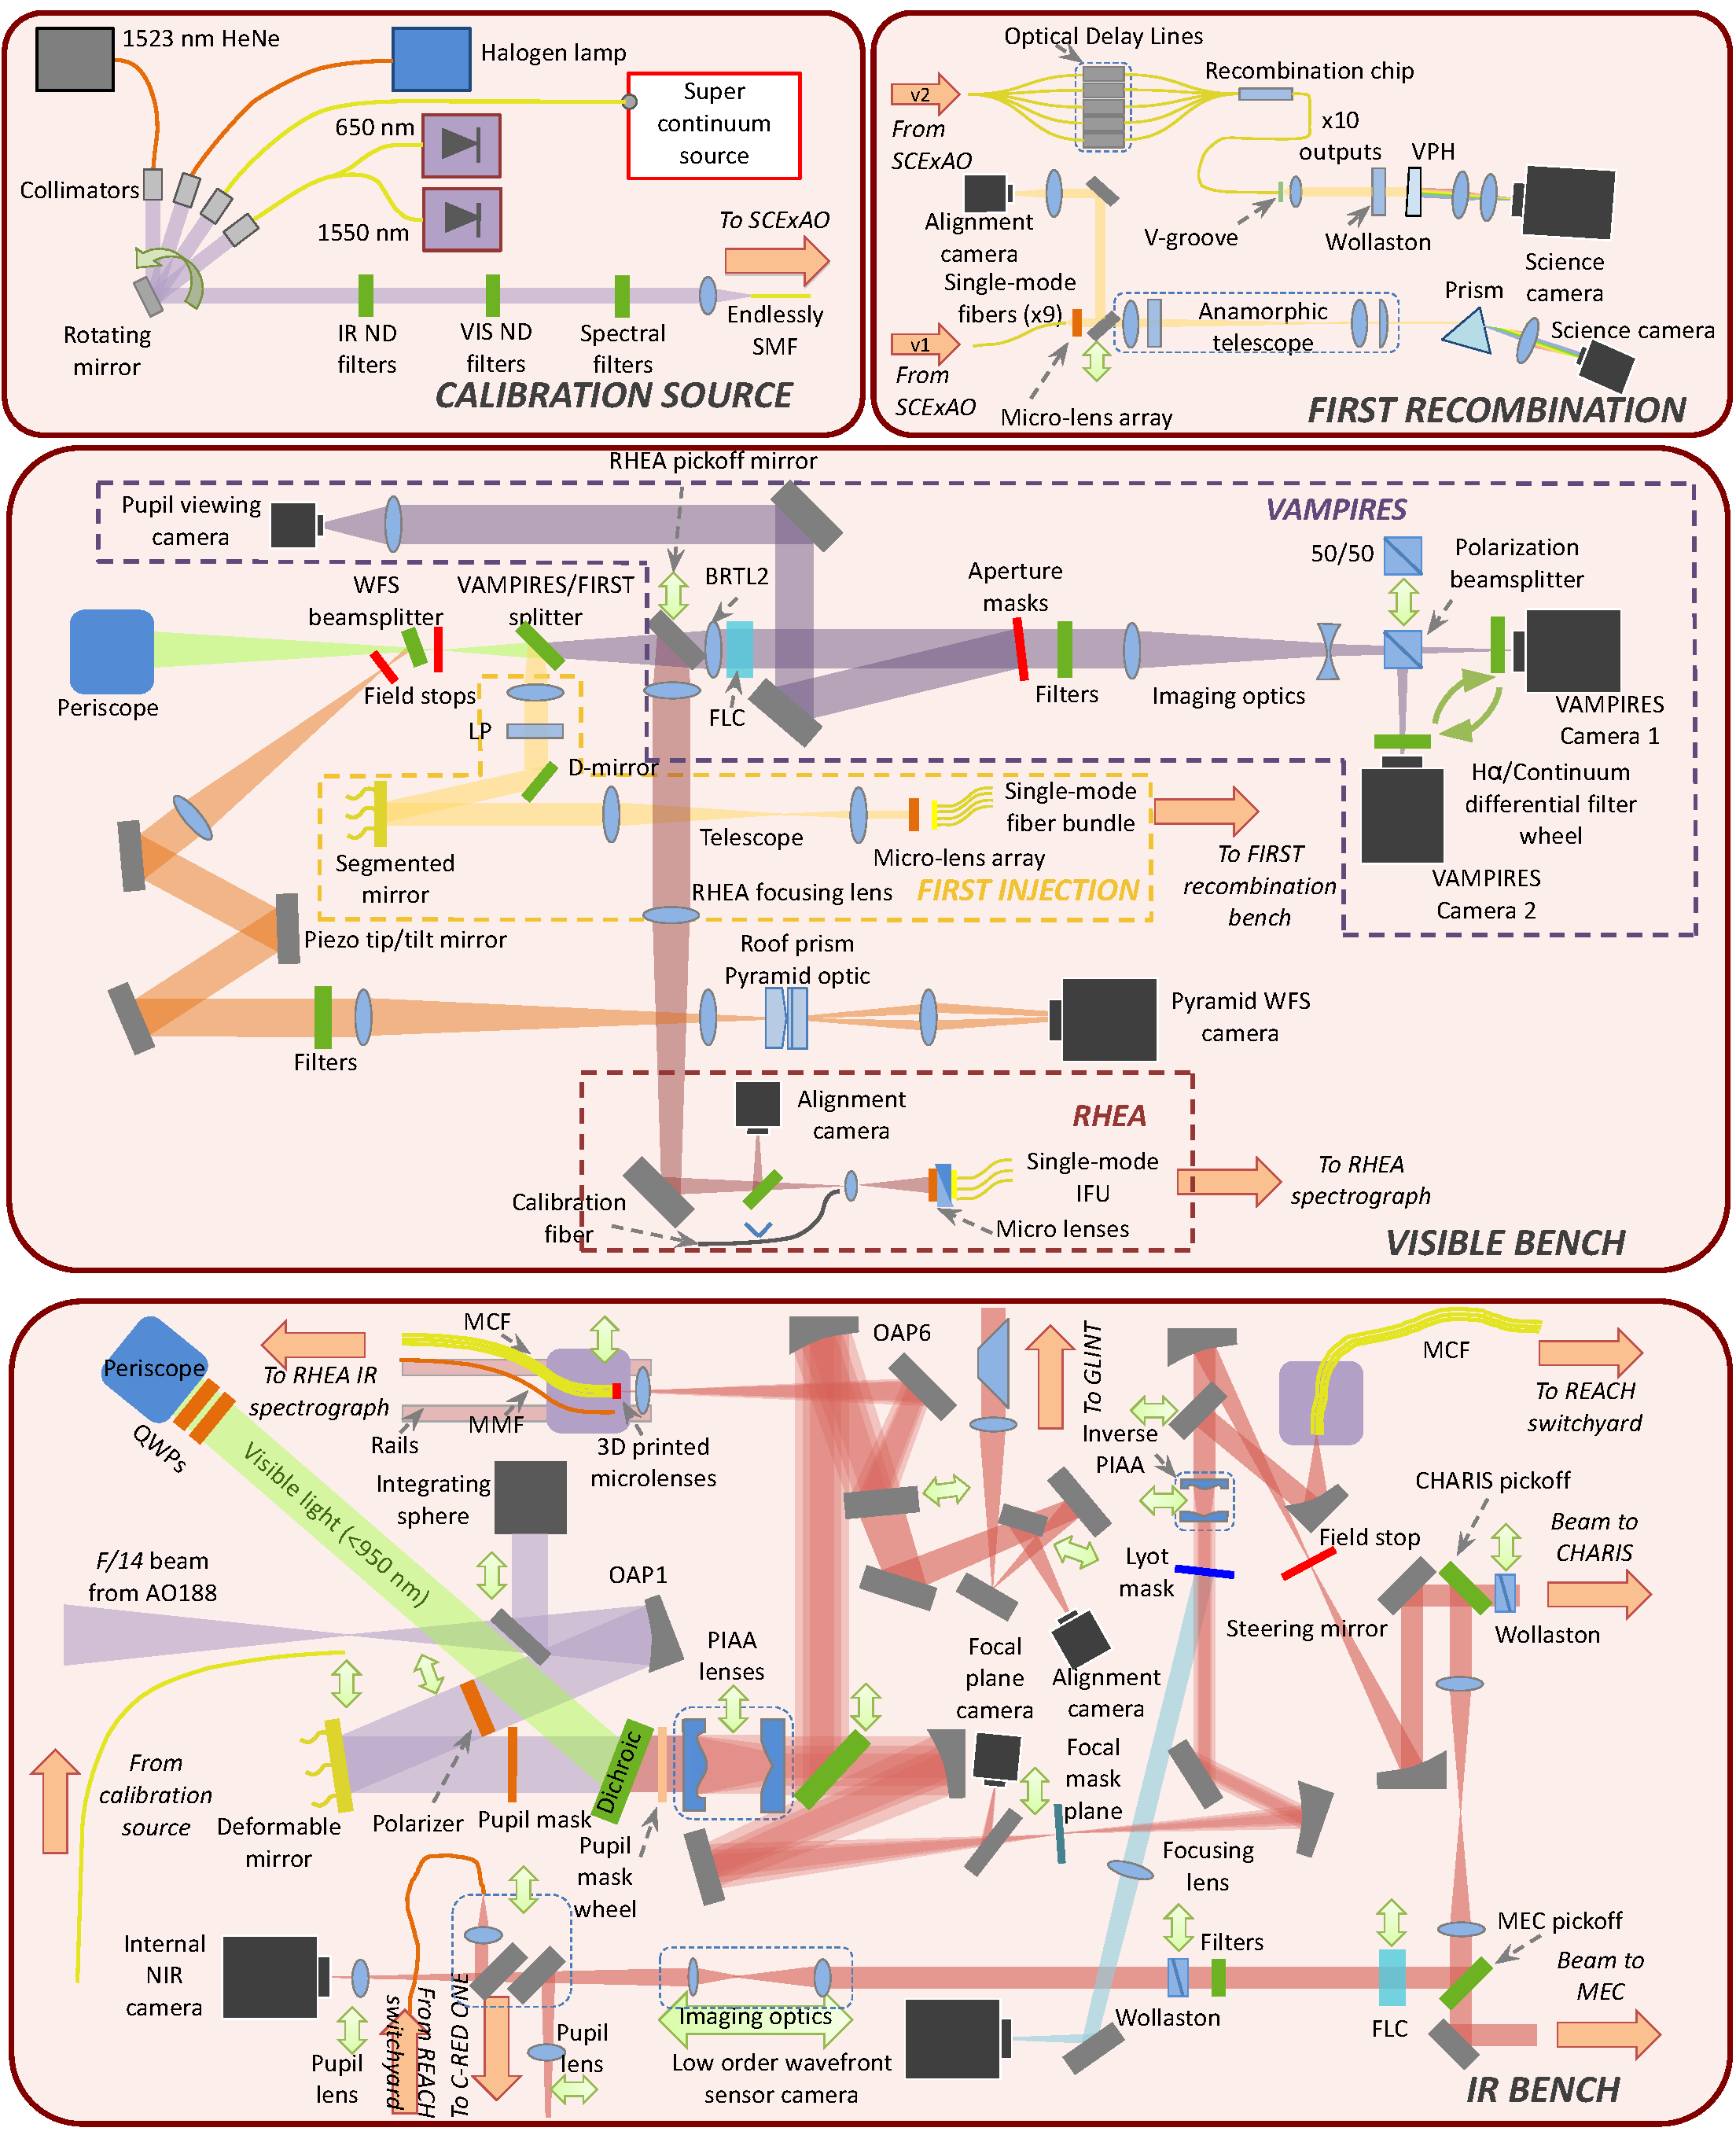
\includegraphics[width=\figwidth]{Figure_Chap5/20230212_FullBench.pdf}
    \caption[Schéma de principe de la plateforme SCExAO.]{Schéma de principe de la plateforme SCExAO. Crédit : équipe SCExAO.}
    \label{fig:SCExAOScheme}
\end{figure}

% 


%%%%%%%%%%%%%%%%%%%%%%%%%%%%%%%%
\section{Intégration de FIRSTv2 à SCExAO}
% Camera bought for FIRST on SCExAO
% Meetings with Hamamatsu: the Orca Quest qCMOS camera is probably the one we want for FIRST. Latest sCMOS. https://www.hamamatsu.com/eu/en/product/type/C15550-20UP/index.html
% Fast mode 0.4 e ron (18Hz, USB), low mode 0.25 e ron (5 Hz).
% Dark current is lower than the previous one: 0.006 e-/pix/sec (water cooled). 
% QE 90% at 475nm, 80% at 600nm, 65% at 700nm.
% 4000x2300 pixels with pixel size 4.6 micron. 
% Price: 45k$

%%%%%%%%%%%%%%%%
\subsection{La cohabitation avec FIRSTv1}
\label{sec:V1V2Subaru}
% intégration des ODLs
% intégration des puces
% intégration du nouveau spectrographe
% d'abord imagée sur la caméra Andor Ixon ---> étude de sensibilité à R=300
% intégration de la caméra hamamatsu (voir com plus haut) --> deux bras independant

% Schéma du banc de recombinaison avant et parès intégration de V2
\begin{figure}[ht!]
    \centering
    \begin{subfigure}{\textwidth}
        \centering
        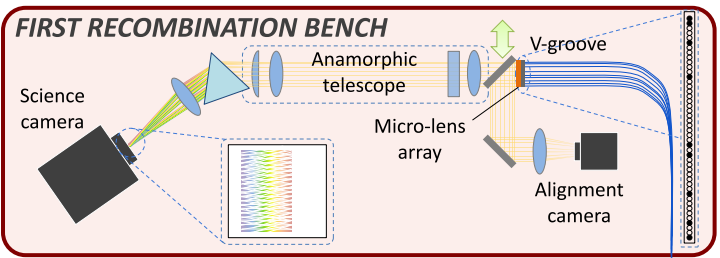
\includegraphics[width=0.95\textwidth]{Figure_Chap5/20230211_FIRST_Recomb_V1_Sheme.png}
    \end{subfigure}
    \begin{subfigure}{\textwidth}
        \centering
        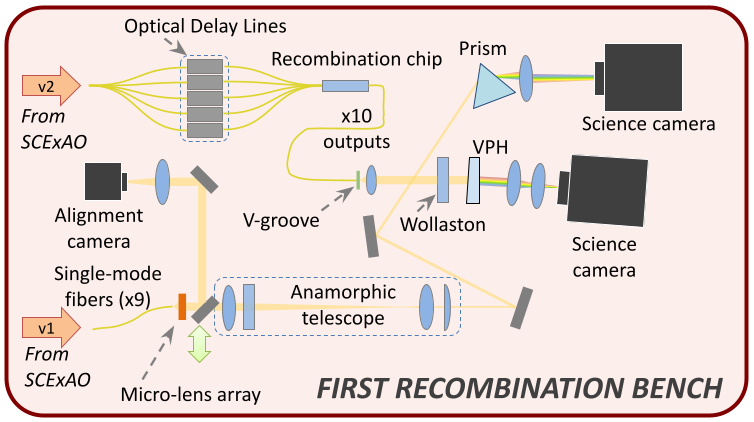
\includegraphics[width=\textwidth]{Figure_Chap5/20220601_SCExAO_FIRSTRecombBench_V1_V2_Scheme.png}
    \end{subfigure}
    \caption[]{Crédit : Sébastien Vievard.}
    \label{fig:FIRSTSubaruScheme}
\end{figure}

% Photo du banc avec les deux versions de FIRST
\begin{figure}[ht!]
    \centering
    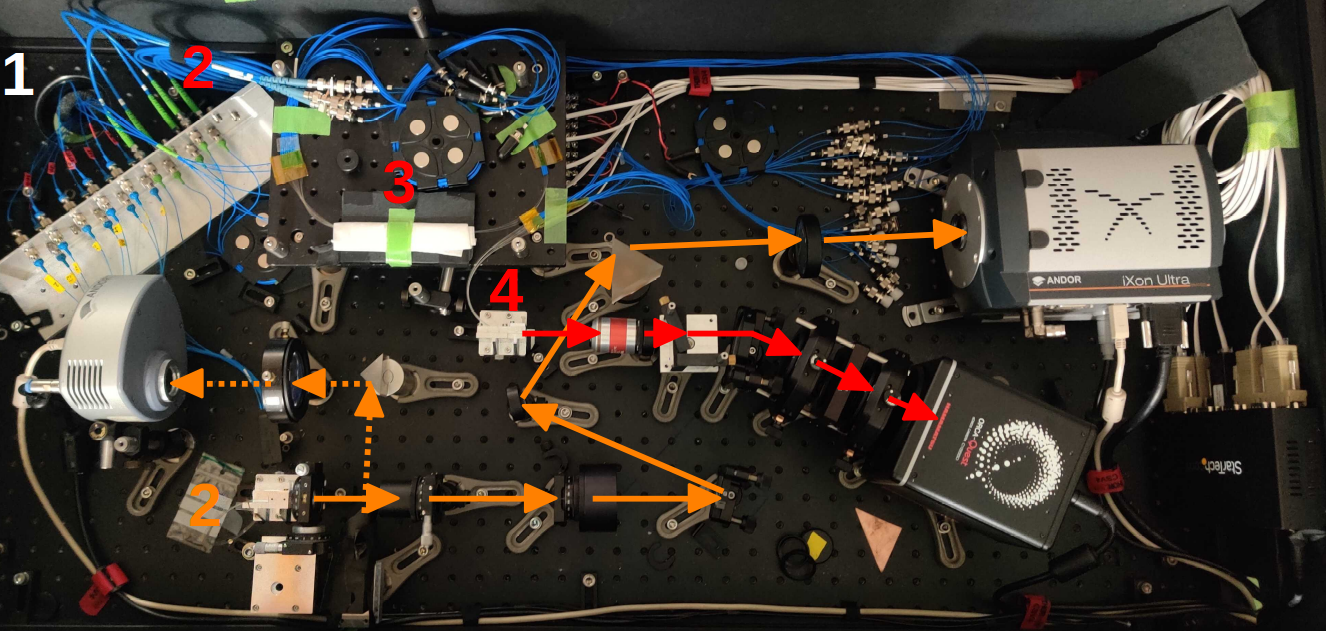
\includegraphics[width=\figwidth]{Figure_Chap5/20220601_SCExAO_FIRSTRecombBench_V1_V2_Photo_label.png}
    \caption[]{Crédit : Sébastien Vievard.}
    \label{fig:FIRSTSubaruPhoto}
\end{figure}


%%%%%%%%%%%%%%%%
\subsection{L'intégration du nouveau spectrographe}
% calcul de la résolution spectrale avec la taille des pixels de la caméra hamamatsu
% trouver une calib spectrale


%%%%%%%%%%%%%%%%
\subsection{La configuration des bases}


\begin{figure}[ht!]
    \centering
    \begin{subfigure}[t]{0.43\textwidth}
        \centering
        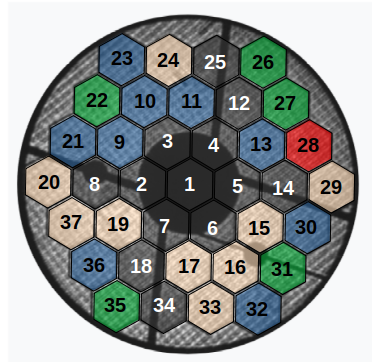
\includegraphics[width=\textwidth]{Figure_Chap5/BaselineMap_Subaru_V1_V2_20221010.png}
        \caption{Configuration des sous-pupilles choisies pour FIRSTv1 (en beige) et FIRSTv2 (en vert) dans le plan pupille du MEMS de FIRST au Subaru. Les segments en noirs sont inutilisés (à cause de l'obstruction centrale, montrée en arrière plan), en rouge est dysfonctionnel et en bleus sont disponibles. Crédit : Sébastien Vievard.}
        \label{fig:SegUVSubaruB}
    \end{subfigure}\hfill
    \begin{subfigure}[t]{0.55\textwidth}
        \centering
        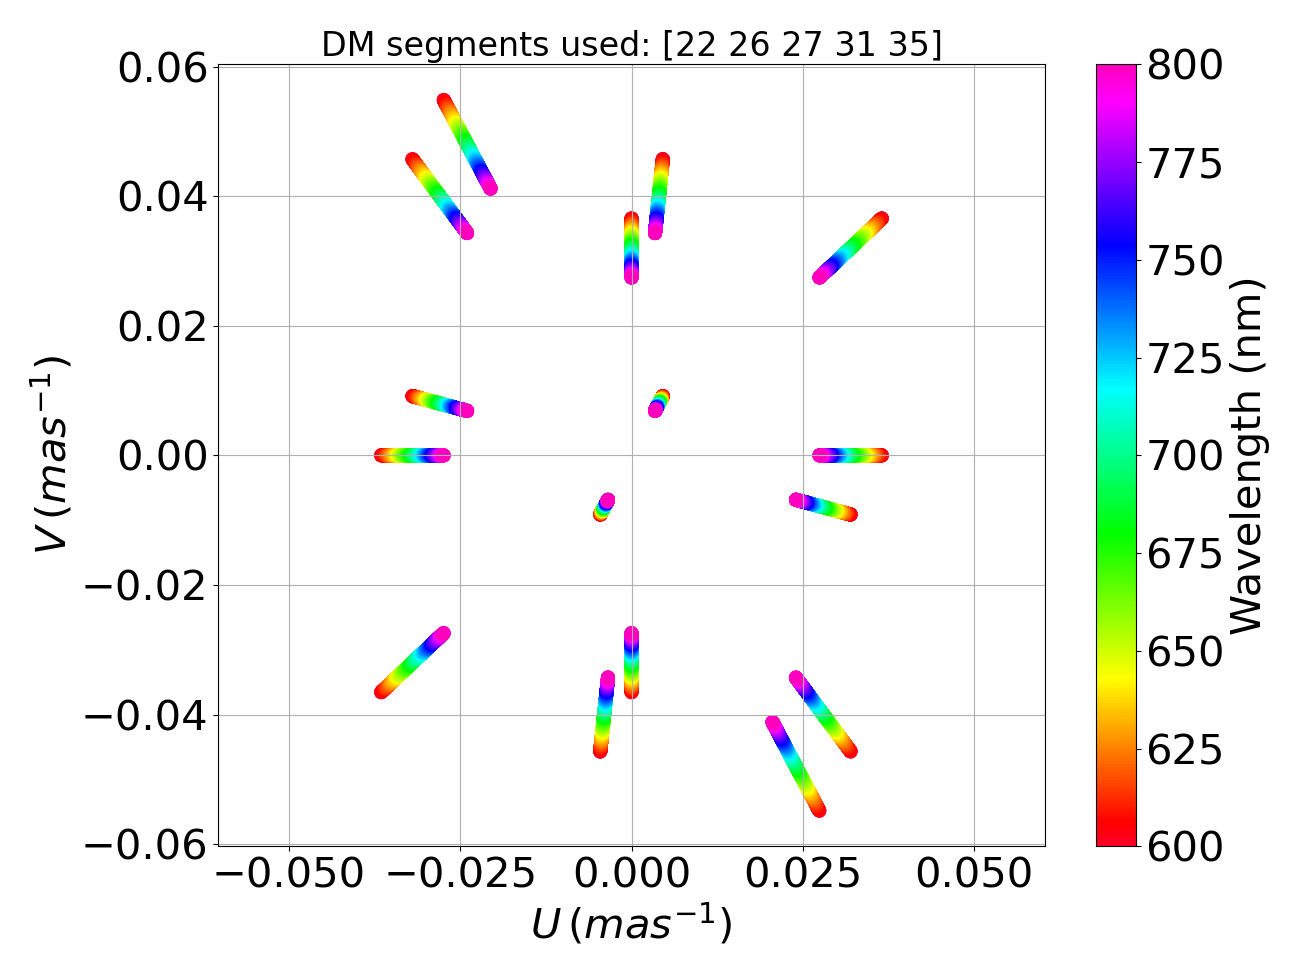
\includegraphics[width=\textwidth]{Figure_Chap5/UVplane_Subaru_22_26_27_31_35.png}
        \caption{La répartition des bases choisies représentée dans l'espace de Fourier, appelée aussi la couverture du plan UV des fréquences spatiales. Les couleurs représentent la longueur d'onde.}
        \label{fig:SegUVSubaruA}
    \end{subfigure}
    \caption[Configuration des sous-pupilles et couverture du plan UV de FIRSTv1 et FIRSTv2 au Subaru.]{Configuration des sous-pupilles et couverture du plan UV de FIRSTv1 et FIRSTv2 au Subaru.}
    \label{fig:SegUVSubaru}
\end{figure}


%%%%%%%%%%%%%%%%%%%%%%%%%%%%%%%
\section{Première lumière au télescope Subaru}

%%%%%%%%%%%%%%%%
\subsection{Les observations}
% tableau des observations et des cibles

%%%%%%%%%%%%%%%%
\subsection{Les résultats préliminaires}

%%%%%%%%%%%%%%%%
\subsection{La sensibilité de FIRSTv2 aux perturbations du banc}
% mesure de la stabilité en fonction du temps sur scexao (pb des franges qui bougent trop vite)
% mesures de phases et de CP ?


%%%%%%%%%%%%%%%%%%%%%%%%%%%%%%%%
\section{Prospectives}
% nouveau DM BMC
% nouvel ordinateur pour la modulation des franges à haute fréquence
% développement d'un nouveau logiciel pour établir un lien avec \ac{CACAO} \citep{guyon2020} le logiciel de calcule temps réel de \ac{SCExAO}, notamment utilisé pour l'OA
% à terme pour la modulation des franges à haute fréquence
